\documentclass[12pt, a4paper]{article}

\usepackage[czech]{babel}
\usepackage{lmodern}
\usepackage[utf8]{inputenc}
\usepackage[T1]{fontenc}
\usepackage[pdftex]{graphicx}
\usepackage{amsmath}
\usepackage[hidelinks,unicode]{hyperref}
\usepackage{float}
\usepackage{listings}
\usepackage{tikz}
\usepackage{xcolor}
\usepackage{tabularx}
\usepackage[final]{pdfpages}
\usepackage{syntax}


\definecolor{mauve}{rgb}{0.58,0,0.82}
\usetikzlibrary{shapes,positioning,matrix,arrows}

\newcommand{\img}[1]{(viz obr. \ref{#1})}

\definecolor{pblue}{rgb}{0.13,0.13,1}
\definecolor{pgreen}{rgb}{0,0.5,0}
\definecolor{pred}{rgb}{0.9,0,0}
\definecolor{pgrey}{rgb}{0.46,0.45,0.48}

%define Javascript language
\lstdefinelanguage{JavaScript}{
keywords={typeof, new, true, false, catch, function, return, null, catch, switch, var, if, in, while, do, else, case, break},
keywordstyle=\color{blue}\bfseries,
ndkeywords={class, export, boolean, throw, implements, import, this},
ndkeywordstyle=\color{darkgray}\bfseries,
identifierstyle=\color{black},
sensitive=false,
comment=[l]{//},
morecomment=[s]{/*}{*/},
commentstyle=\color{purple}\ttfamily,
stringstyle=\color{pgreen}\ttfamily,
morestring=[b]',
morestring=[b]"
}


\lstdefinelanguage{json}{
    basicstyle=\normalfont\ttfamily,
    commentstyle=\color{eclipseStrings}, % style of comment
    stringstyle=\color{eclipseKeywords}, % style of strings
    numbers=left,
    numberstyle=\scriptsize,
    stepnumber=1,
    numbersep=8pt,
    showstringspaces=false,
    breaklines=true,
    frame=lines,
    string=[s]{"}{"},
    comment=[l]{:\ "},
    morecomment=[l]{:"},
    literate=
        *{0}{{{\color{numb}0}}}{1}
         {1}{{{\color{numb}1}}}{1}
         {2}{{{\color{numb}2}}}{1}
         {3}{{{\color{numb}3}}}{1}
         {4}{{{\color{numb}4}}}{1}
         {5}{{{\color{numb}5}}}{1}
         {6}{{{\color{numb}6}}}{1}
         {7}{{{\color{numb}7}}}{1}
         {8}{{{\color{numb}8}}}{1}
         {9}{{{\color{numb}9}}}{1}
}

\lstset{
    frame=tb,
    language=json,
    aboveskip=3mm,
    belowskip=3mm,
    showstringspaces=false,
    columns=flexible,
    basicstyle={\small\ttfamily},
    numbers=none,
    numberstyle=\tiny\color{gray},
    keywordstyle=\color{blue},
    commentstyle=\color{pgreen},
    stringstyle=\color{mauve},
    breaklines=true,
    breakatwhitespace=true,
    tabsize=3
}

\lstset{language=SQL,morekeywords={PREFIX,FILTER,java,rdf,rdfs,url}}


\let\oldsection\section
\renewcommand\section{\clearpage\oldsection}

\begin{document}
	% this has to be placed here, after document has been created
	% \counterwithout{lstlisting}{chapter}
	\renewcommand{\lstlistingname}{Ukázka kódu}
	\renewcommand{\lstlistlistingname}{Seznam ukázek kódu}
    \begin{titlepage}

        \centering

        \vspace*{\baselineskip}
        \begin{figure}[H]
        \centering
        
\includegraphics[width=7cm]{img/fav-logo.jpg}
        \end{figure}

        \vspace*{1\baselineskip}

        \vspace{0.75\baselineskip}

        \vspace{0.5\baselineskip}
        {Semestrální práce z předmětu KIV/DB2}

        {\LARGE\sc RDF databáze a SPARQL dotazy\\}

        \vspace{4\baselineskip}

        \vspace{0.5\baselineskip}

        {\sc\Large Stanislav Král \\}
        \vspace{0.5\baselineskip}
        {A20N0091P}

        \vfill

        {\sc Západočeská univerzita v Plzni\\
        Fakulta aplikovaných věd}

    \end{titlepage}


    % TOC
    \tableofcontents
    \pagebreak

    
\section{Popis řešeného tématu}
Zvolené téma představuje situaci investora, který nakupuje a prodává kryptoměny na různých směnárnách či burzách. Pro takového investora je důležité, aby všechny informace o nákupech byly jednoduše dohledatelné a aby jednotlivé kryptoměny mohl třídit do portfólií. Tento investor by si mohl například chtít třídit nákupy do portfólia, ve kterém si bude vést obchody s významnějšími kryptoměnami (např. Bitcoin či Ethereum) a obchody s méně významnými kryptoměnami (dle tržní kapitalizace např. Basic Attention Token či Solana) do jiného portfólia.
    
Dále je také nutné, aby ke každému obchodu byla přiřazena informace v jaké měně byl uskutečněn. Toto se nejčastěji reprezentuje pomocí tzv. \textit{obchodních párů}, které se skládají z měny (např. USD) a dané komodity (např. BTC).

Pomocí takto popsaného nástroje (databáze), který tento problém řeší, si investor může např. svá portfólia porovnat oproti aktuálnímu kurzu kryptoměn, a zjistit jak se jeho obchodům daří. Takový nástroj by také našel využití i při vyplňování daňového přiznání.

\section{Popis datové struktury}

Ve vytvořené databází se používají následující jmenné prostory:

\begin{itemize}
    \item \texttt{http://kralst.cz/ontologies/crypto/portfolio} -- jmenný prostor portfólií
    \item \texttt{http://kralst.cz/ontologies/crypto/tradingPair} -- jmenný prostor obchodních párů
    \item \texttt{http://kralst.cz/ontologies/crypto/order} -- jmenný prostor transakcí
    \item \texttt{http://kralst.cz/ontologies/prop} -- jmenný prostor určený pro popis vlastností entit vyskytujících se v databázi
    \item \texttt{http://kralst.cz/ontologies/type} -- jmenný prostor pro specifikaci typů entit vyskytujících se v databázi
\end{itemize}

Základní vazba mezi entitami datové struktury je taková, že transakce referencuje jak portfólio, do kterého je zařazena, tak i obchodní pár, kterého se týká. Pomocí transakcí je realizována vazba M:N mezi portfóliemi a kryptoměnami (součást obchodního páru).

\begin{figure}[!ht]
\centering
{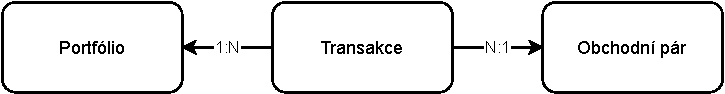
\includegraphics[width=13.5cm]{img/diagram.pdf}}
\caption{Diagram zobrazující základní relace mezi objekty dat. struktury}
\label{fig:screen-transition-diagram}
\end{figure}

Pro splnění zadání byla k některým portfóliím uměle přidána informace, jaké transakce do něj patří.

\subsection{Portfólia}
Objekty typu \texttt{Portfolio} představují portfólia a mívají následující vlastnosti:
\begin{itemize}
    \item \texttt{name} -- pojmenování portfólia
    \item \texttt{description} -- vlastní popis portfólia
    \item \texttt{transactions} -- seznam vybraných transakcí, které jsou k portfóliu přiřazeny (neobjevuje se vždy)
\end{itemize}

\begin{lstlisting}
portfolio:1 a                   type:Portfolio ;
             prop:name           "Main portfolio" ;
             prop:description    "Tracking Bitcoin/Ethereum" .
\end{lstlisting}

\subsection{Obchodní páry}
Pro reprezentaci obchodních párů, které byly kdy obchodovány, se používají objekty typu \texttt{TradingPair} mající následující vlastnosti:

\begin{itemize}
    \item \texttt{symbol} -- zkratka kryptoměny
    \item \texttt{name} -- celý název kryptoměny
    \item \texttt{currency} -- zkratka měny, ve které je daná kryptoměna obchodována
\end{itemize}

\begin{lstlisting}
tradingPair:1   a               type:TradingPair ;
                prop:symbol     "BTC" ;
                prop:name       "Bitcoin" ;
                prop:currency   "USD" .
\end{lstlisting}


\subsection{Uskutečněné obchody (transakce)}
Aby bylo možné ukládat informaci o uskutečněných obchodech, tak se vytváří objekty typu \texttt{Order}, které obsahují následující atributy popisující vlastnosti transakce: 
\begin{itemize}
    \item \texttt{size} -- množství kryptoměny, která byla obchodována
    \item \texttt{price} -- cena za jednu minci kryptoměny
    \item \texttt{fee} -- poplatek za uskutečněný nákup
    \item \texttt{timestamp} -- datum a čas, kdy se nákup uskutečnil ve formátu UNIX Timestamp
    \item \texttt{tradingPair} -- obchodní pár, kterého se tento obchod týkal
    \item \texttt{sell} -- nepovinná vlastnost, která se nastavuje na objekt \texttt{true}, pokud daný obchod představoval prodej
    \item \texttt{portfolio} -- portfólio, do kterého daný obchod patří
\end{itemize}

\begin{lstlisting}
order:2     a                   type:Order ;
            prop:size           0.30 ;
            prop:price          20900 ;
            prop:fee            0.22 ;
            prop:timestamp      1618675531 ;
            prop:tradingPair    tradingPair:1 ;
            prop:sell           true ;
            prop:portfolio      portfolio:1 .
\end{lstlisting}

\section{Popis vyhledávacích dotazů nad databázovou strukturou}
Ke zjištení užitečných informací o obchodování bylo vytvořeno 7 dotazů.

\subsection{Vyhledání všech nákupů portfólia o větším než požadovaném objemu  }
Pro vyhledání všech nákupních transakcí, které jsou přiřazeny vybranému portfóliu a obchodovaly větší než požadovaný objem krpytoměny, slouží následující dotaz:

\begin{lstlisting}
PREFIX type: <http://kralst.cz/ontologies/type#>
PREFIX portfolio: <http://kralst.cz/ontologies/crypto/portfolio#>
PREFIX prop: <http://kralst.cz/ontologies/prop#>

SELECT  *

WHERE {
  ?order a type:Order .
  ?order prop:portfolio portfolio:1 .
  ?order prop:size ?size .
  FILTER NOT EXISTS {
  	?order prop:sell true
  }
  
  FILTER (
  	?size > 0.010
  )
}
\end{lstlisting}
Výsledek obsahuje jednotlivé nákupy a jejich objemy.

\subsection{Vyhledání všech obchodních párů, které mají v názvu vybraný podřetězec}
Seznam všech obchodních párů, které v názvu obsahují požadovaný podřetězec, lze získat vykonáním následujícího dotazu:

\begin{lstlisting}
PREFIX portfolio: <http://kralst.cz/ontologies/crypto/tradingPair#>
PREFIX type: <http://kralst.cz/ontologies/type#>
PREFIX prop: <http://kralst.cz/ontologies/prop#>

SELECT  *

WHERE {
    ?tradingPair a type:TradingPair .
    ?tradingPair prop:symbol ?symbol .
    ?tradingPair prop:name ?name .

    FILTER(
        # trading pairs containing the string "coin" in their name
        regex(?name, "coin")
    
}
\end{lstlisting}
Výsledek obsahuje jednotlivé obchodní páry, zkratku kryptoměny a její název.

\subsection{Vyhledání všech uskutečněných prodejů}
Seznam všech prodejů včetně názvu portfólií, ve kterých se uskutečnily, lze získat vykonáním následujícího dotazu:

\begin{lstlisting}
PREFIX type: <http://kralst.cz/ontologies/type#>
PREFIX prop: <http://kralst.cz/ontologies/prop#>

SELECT  ?portfolioName ?size ?symbol

WHERE {
  	?order a type:Order .
  	?order prop:portfolio ?portfolio .
  	?portfolio prop:name ?portfolioName .
  	?order prop:tradingPair/prop:symbol ?symbol .
  	?order prop:size ?size .
  	?order prop:sell true
}

\end{lstlisting}
Každý řádek výsledku dotazu se skládá z názvu portfólia, ve kterém byl uskutečněn daný prodej, objemu transakce a zkratky kryptoměny, které se transakce týkala.


\subsection{Vyhledání všech transakcí uskutečněných ve vybrané měně}
K získání seznamu všech transakcí, které se uskutečnily ve vybrané měně, lze použít následující dotaz:

\begin{lstlisting}
PREFIX prop: <http://kralst.cz/ontologies/prop#>

SELECT  *

WHERE {
	    "EUR"	^prop:currency/^prop:tradingPair ?order.
                ?order			prop:price			?price.
                ?order			prop:size			?size;
}
\end{lstlisting}
Každý řádek výsledku dotazu se skládá z nalezené transakce, ceny za jednu minci obchodované kryptoměny a počet obchodovaných mincí.

Tento dotaz využívá dvakrát syntax pro vyhledání inverzní hrany, a to z toho důvodu, že chceme nalézt všechny obchodní páry s vybranou měnou, a poté všechny transakce, které se týkaly již nalezených párů.


\subsection{Výpočet sumy všech poplatků za uskutečněné transakce napříč jednotlivými portfólii}
K vypočtení sumy všech poplatků za uskutečněné transakce napříč jednotlivými portfóliemi lze použít následující dotaz obsahující agregaci:

\begin{lstlisting}
PREFIX prop: <http://kralst.cz/ontologies/prop#>
PREFIX type: <http://kralst.cz/ontologies/type#>


SELECT  (SUM(?fee) as ?feeSum) ?name

WHERE {
    ?order	a type:Order .
    ?order prop:portfolio ?portfolio .
    ?order prop:fee ?fee .
    ?portfolio prop:name ?name .
}

GROUP BY ?portfolio	?name

\end{lstlisting}

Jednotlivé řádky výsledku se poté skládají z názvu portfólia a sumy všech poplatků za transakce k němu přiřazené.


\subsection{Vyhledání všech transakcí týkajících se vybraných kryptoměn}
Následující dotaz slouží k vyhledání všech transakcí, v rámci kterých byl uskutečněn obchod s vybranými kryptoměnami:

\begin{lstlisting}
PREFIX prop: <http://kralst.cz/ontologies/prop#>


SELECT  ?portfolioName ?symbol ?size ?price

WHERE {
    VALUES ?symbol {"LTC" "ETH" "ADA"}

    ?tradingPair prop:symbol ?symbol .

    ?tradingPair ^prop:tradingPair	?order .

    ?order prop:size	?size .
    ?order prop:price	?price .

    ?order prop:portfolio/prop:name ?portfolioName .
}

\end{lstlisting}

Řádky výsledku se skládají z názvu portfólia, ve kterém byla uskutečněna hledaná transakce, ze zkratky kryptoměny, objemu transakce a ceny za jednu minci kryptoměny.


\subsection{Vyhledání všech transakcí týkajících se vybraných kryptoměn o minimální požadované hodnotě}
Jako alternativní dotaz pro vyhledání všech transakcí týkajících se vybraných kryptoměn doplněný o požadavek na minimální hodnotu transakce lze použít následující dotaz:

\begin{lstlisting}
PREFIX type: <http://kralst.cz/ontologies/type#>
PREFIX prop: <http://kralst.cz/ontologies/prop#>

SELECT  *

WHERE {
  	?order a type:Order .
  	?order prop:size ?size .
  	?order prop:price	?price .
  
  	?order prop:tradingPair/prop:symbol ?symbol .
  	?order prop:tradingPair/prop:currency ?currency .

	BIND (?price * ?size AS ?cost) 
    
  	FILTER (
    	?cost > 1500  && (?symbol = "BTC" || ?symbol = "LTC")
    )
}
\end{lstlisting}

Řádky výsledku se skládají z transakce, objemu transakce, ceny za jednu minci, zkratku obchodované kryptoměny, měny, ve které byla uskutečněna daná transakce a hodnoty transakce.

Hodnota transakce je vypočtena vynásobením objemu transakce a ceny za jednu minci kryptoměny.


\subsection{Vyhledání všech transakcí ve vybraném portfóliu s využitím hran vedoucích do transakcí}
Jako demonstrace využití hran vedoucích do transakcí (cyklus transakce/portfólia) slouží následující dotaz pro vyhledání všech transakcí vybraného portfólia:

\begin{lstlisting}
PREFIX portfolio: <http://kralst.cz/ontologies/crypto/portfolio#>
PREFIX prop: <http://kralst.cz/ontologies/prop#>

SELECT  ?size ?price ?symbol

WHERE {
  portfolio:3	prop:orders						?order.
  ?order		prop:size 						?size.
  ?order		prop:price 						?price.
  ?order		prop:tradingPair/prop:symbol 	?symbol.
}
\end{lstlisting}

Řádky výsledku se skládají z objemu transakce, ceny za jednu minci a zkratky obchodované kryptoměna.


\section{Diskuze nad řešením v dané technologii}
Navržený model by šlo rozčlenit do více souborů, kdy by byly oddělené definice objektů jednotlivých typů entit. Bylo by však třeba správně ve všech souborech používat vytvořené jmenné prostory.

Navzdory prvním pocitům z této databázové technologie jsem nenarazil na žádnou limitaci formátu RDF pro uložení dat z domény vedení záznamů o obchodování s kryptoměnami. Naopak jsem byl příjemně překvapen čitelným formátem TTL a jednoduchým (avšak mocným) dotazovacím jazykem SPARQL, kdy jsem nenarazil na žádnou obtíž při vytváření dotazů. Velmi pohodlná je syntax \textit{Property Path}

Při využití konstrukce \texttt{OPTIONAL}, \texttt{FILTER NOT EXISTS} či chytré definice trojic při sestavování dotazu jsou nepovinné vlastnosti typu \texttt{sell} označující transakce, které představují prodej, bezproblémové.

V případě modelování databázové struktury při řešení problému sledování uskutečněných obchodů s kryptoměnami nevidím příliš velké využití zápisu relace mezi 2 uzly pomocí 2 hran (oba směry), a tak se mi ani nepodařilo vymyslet nějaký užitečný cyklus v grafu modelu. Současný navržený model, řekl bych, že dobře řeší zmíněný problém, a tak např. hrany vedoucí z uzlů portfólií do uzlů transakcí nepřinášejí žádnou přidanou hodnotu. 



\end{document} 
